\documentclass[xetex,mathserif,serif]{beamer}
\usepackage{polyglossia}
\setdefaultlanguage[babelshorthands=true]{russian}
\usepackage{minted}
\usepackage{tabu}

\useoutertheme{infolines}

\usepackage{fontspec}
\setmainfont{FreeSans}
\newfontfamily{\russianfonttt}{FreeSans}

\definecolor{links}{HTML}{2A1B81}
\hypersetup{colorlinks,linkcolor=,urlcolor=links}

\tabulinesep=0.7mm

\newcommand{\attribution}[1] {
    \vspace{-5mm}\begin{flushright}\begin{scriptsize}\textcolor{gray}{\textcopyright\, #1}\end{scriptsize}\end{flushright}
}

\title{Практика 10: примеры архитектур}
\subtitle{Системы контроля версий}
\author[Юрий Литвинов]{Юрий Литвинов \newline \textcolor{gray}{\small\texttt{yurii.litvinov@gmail.com}}}

\date{21.03.2022}

\begin{document}
    
\frame{\titlepage}

    \section{Введение}

    \begin{frame}
        \frametitle{Краткая история систем контроля версий}
        \begin{itemize}
            \item 1975 -- SCCS (Source Code Control System)
            \begin{itemize}
                \item Дельты
            \end{itemize}
            \item 1982 -- RCS (Revision Control System)
            \begin{itemize}
                \item С открытым исходным кодом (до сих пор поддерживается GNU)
            \end{itemize}
            \item 1986 -- CVS (Concurrent Versioning System)
            \begin{itemize}
                \item Одновременное редактирование, мерджи, ветки, тэги, удалённые репозитории
            \end{itemize}
            \item 2000 -- SVN (Subversion)
            \item 2005 --- Git, Mercurial, Bazaar
            \begin{itemize}
                \item Распределённые
            \end{itemize}
        \end{itemize}
    \end{frame}

    \section{Git}

    \begin{frame}
        \frametitle{Git\footnote{\tiny{По гл. 10 \url{https://git-scm.com/book} и \url{http://aosabook.org/en/git.html}}}}
        \begin{itemize}
            \item Распределённая VCS
            \item Linus Torvalds, 2005 год, драма с BitKeeper
            \item Architectural drivers
            \begin{itemize}
                \item Распределённая разработка с тысячей коммитеров
                \item Защита от порчи исходников
                \begin{itemize}
                    \item Возможность отменить мердж, смерджиться вручную
                \end{itemize}
                \item Высокая скорость работы
            \end{itemize}
        \end{itemize}
    \end{frame}

    \begin{frame}
        \frametitle{Внутреннее устройство Git}
        Структура папки .git:
        \begin{itemize}
            \item HEAD
            \item index
            \item config
            \item description
            \item hooks/
            \item info/
            \item objects/
            \item refs/
            \item ...
        \end{itemize}
    \end{frame}

    \begin{frame}[fragile]
        \frametitle{Объекты}
        Git внутри --- хеш-таблица, отображающая SHA-1-хеш файла в содержимое файла. Пример:
        \begin{minted}{text}
$ git init test
Initialized empty Git repository in /tmp/test/.git/
$ cd test
$ find .git/objects
.git/objects
.git/objects/info
.git/objects/pack

$ echo 'test content' | git hash-object -w --stdin
d670460b4b4aece5915caf5c68d12f560a9fe3e4

$ find .git/objects -type f
.git/objects/d6/70460b4b4aece5915caf5c68d12f560a9fe3e4
        \end{minted}
    \end{frame}

    \begin{frame}[fragile]
        \frametitle{Объекты (2)}
        Как получить сохранённый объект:
        \begin{minted}{text}
$ git cat-file -p d670460b4b4aece5915caf5c68d12f560a9fe3e4
test content
        \end{minted}

        Версионный контроль:
        \begin{minted}{text}
$ echo 'version 1' > test.txt
$ git hash-object -w test.txt
83baae61804e65cc73a7201a7252750c76066a30
$ echo 'version 2' > test.txt
$ git hash-object -w test.txt
1f7a7a472abf3dd9643fd615f6da379c4acb3e3a
$ find .git/objects -type f
.git/objects/1f/7a7a472abf3dd9643fd615f6da379c4acb3e3a
.git/objects/83/baae61804e65cc73a7201a7252750c76066a30
.git/objects/d6/70460b4b4aece5915caf5c68d12f560a9fe3e4
        \end{minted}
    \end{frame}

    \begin{frame}[fragile]
        \frametitle{Объекты (3)}
        Переключение между версиями файла:
        \begin{minted}{text}
$ git cat-file -p 83baae61804e65cc73a7201a7252750c76066a30 \
> test.txt
$ cat test.txt
version 1

$ git cat-file -p 1f7a7a472abf3dd9643fd615f6da379c4acb3e3a \
> test.txt
$ cat test.txt
version 2
        \end{minted}
    \end{frame}

    \begin{frame}[fragile]
        \frametitle{Деревья}
        blob (то, что мы видели раньше) хранит только содержимое файла, не хранит даже его имя. Решение проблемы --- tree:
        \begin{scriptsize}
        \begin{minted}{text}
$ git cat-file -p master^{tree}
100644 blob a906cb2a4a904a152e80877d4088654daad0c859      README
100644 blob 8f94139338f9404f26296befa88755fc2598c289      Rakefile
040000 tree 99f1a6d12cb4b6f19c8655fca46c3ecf317074e0      lib
        \end{minted}
        \end{scriptsize}
        \begin{center}
            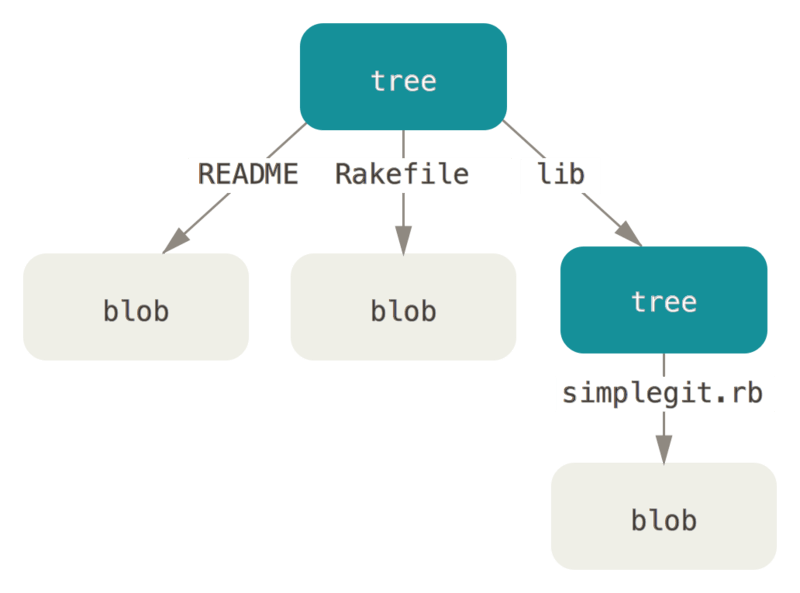
\includegraphics[width=0.5\textwidth]{gitTreeObject.png}
        \end{center}
    \end{frame}

    \begin{frame}
        \frametitle{Какие ещё виды объектов бывают}
        \begin{center}
            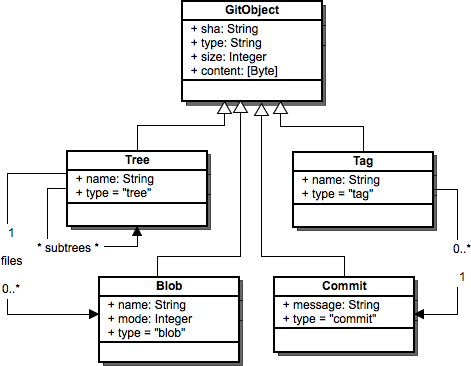
\includegraphics[width=0.7\textwidth]{gitDataStructure.png}
        \end{center}
    \end{frame}

    \begin{frame}[fragile]
        \frametitle{Коммиты}
        tree-объекты могут хранить структуру файлов (как inode в файловой системе), но не хранят метаинформацию типа автора файла и даты создания. Это хранится в commit-объектах:
        \begin{minted}{text}
$ echo 'first commit' | git commit-tree d8329f
fdf4fc3344e67ab068f836878b6c4951e3b15f3d

$ git cat-file -p fdf4fc3
tree d8329fc1cc938780ffdd9f94e0d364e0ea74f579
author Scott Chacon <schacon@gmail.com> 1243040974 -0700
committer Scott Chacon <schacon@gmail.com> 1243040974 -0700

first commit
        \end{minted}
        Ещё коммит хранит список коммитов-родителей
    \end{frame}

    \begin{frame}
        \frametitle{Коммиты, как это выглядит}
        \begin{center}
            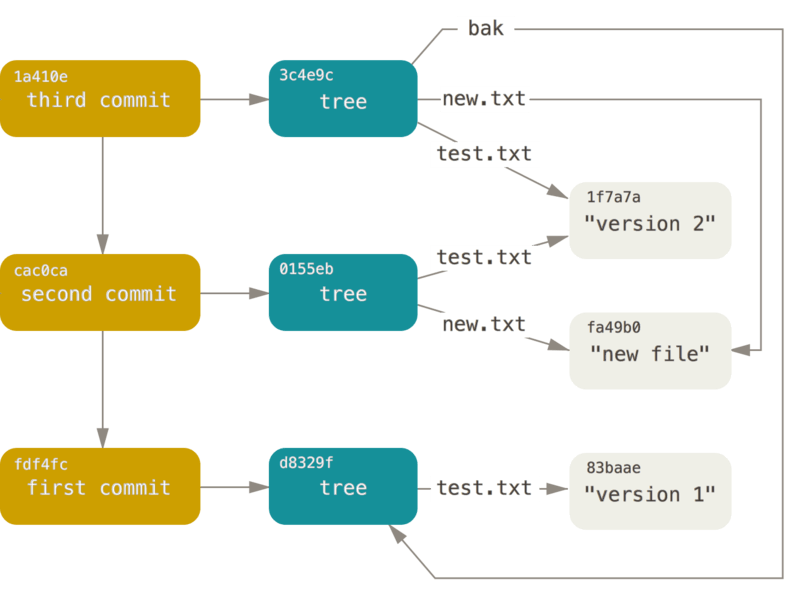
\includegraphics[width=0.7\textwidth]{gitCommitObjects.png}
        \end{center}
    \end{frame}

    \begin{frame}[fragile]
        \frametitle{Ссылки}
        Теперь вся информация хранится на диске, но чтобы ей воспользоваться, нужно помнить SHA-1 хеши. На помощь приходят reference-ы. 

        \begin{itemize}
            \item .git/refs
            \item .git/refs/heads
            \item .git/refs/tags
        \end{itemize}

        \begin{minted}{text}
$ echo "1a410efbd13591db07496601ebc7a059dd55cfe9" \
> .git/refs/heads/master

$ git log --pretty=oneline master
1a410efbd13591db07496601ebc7a059dd55cfe9 third commit
cac0cab538b970a37ea1e769cbbde608743bc96d second commit
fdf4fc3344e67ab068f836878b6c4951e3b15f3d first commit
        \end{minted}
        \begin{itemize}
            \item Команда \verb|git update-ref|
        \end{itemize}
    \end{frame}

    \begin{frame}
        \frametitle{Ссылки, как это выглядит}
        \begin{center}
            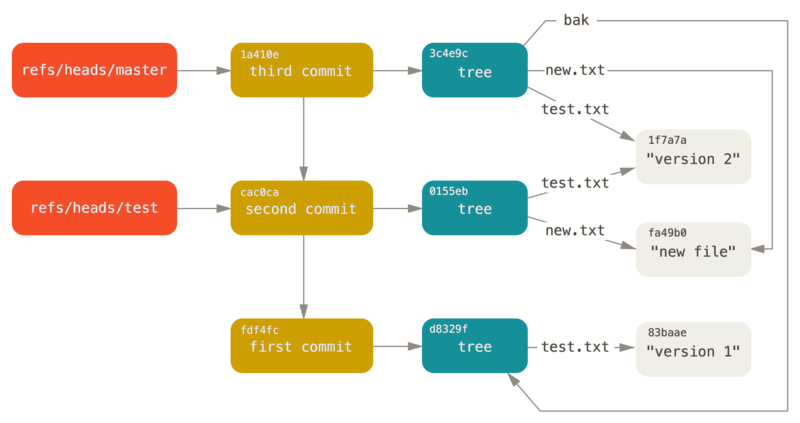
\includegraphics[width=0.9\textwidth]{gitRefs.png}
        \end{center}
    \end{frame}

    \begin{frame}[fragile]
        \frametitle{HEAD}
        Теперь не надо помнить хеши, но как переключаться между ветками?

        Текущая ветка хранится в HEAD. HEAD --- символическая ссылка, то есть ссылка на другую ссылку.
        \begin{minted}{text}
$ cat .git/HEAD
ref: refs/heads/master

$ git symbolic-ref HEAD refs/heads/test
$ cat .git/HEAD
ref: refs/heads/test
        \end{minted}
    \end{frame}

    \begin{frame}[fragile]
        \frametitle{Тэги}
        Последний из объектов в Git --- tag. Это просто указатель на коммит.
        \begin{footnotesize}
            \begin{itemize}
                \item Легковесный тэг:
                    \begin{minted}{text}
git update-ref refs/tags/v1.0 cac0cab538b970a37ea1e769cbbde608743bc96d
                    \end{minted}
                    Или просто git tag
                \item Аннотированный тэг:
                    \begin{minted}{text}
$ git tag -a v1.1 1a410efbd13591db07496601ebc7a059dd55cfe9 -m 'test tag'

$ git cat-file -p 9585191f37f7b0fb9444f35a9bf50de191beadc2
object 1a410efbd13591db07496601ebc7a059dd55cfe9
type commit
tag v1.1
tagger Scott Chacon <schacon@gmail.com> Sat May 23 16:48:58 2009 -0700

test tag
                    \end{minted}
            \end{itemize}
        \end{footnotesize}
    \end{frame}

    \begin{frame}[fragile]
        \frametitle{Packfiles}
        Пока что получалось, что все версии всех файлов в Git хранятся целиком, как они есть. Все они всегда сжимаются zlib, но в целом, если создать репозиторий, добавлять туда файлы, коммитить и т.д., все версии всех файлов будут в нём целиком. На помощь приходят .pack-файлы:
        \begin{footnotesize}
            \begin{minted}{text}
$ git gc
Counting objects: 18, done.
Delta compression using up to 8 threads.
Compressing objects: 100% (14/14), done.
Writing objects: 100% (18/18), done.
Total 18 (delta 3), reused 0 (delta 0)

$ find .git/objects -type f
.git/objects/bd/9dbf5aae1a3862dd1526723246b20206e5fc37
.git/objects/d6/70460b4b4aece5915caf5c68d12f560a9fe3e4
.git/objects/info/packs
.git/objects/pack/pack-978e03944f5c581011e6998cd0e9e30000905586.idx
.git/objects/pack/pack-978e03944f5c581011e6998cd0e9e30000905586.pack
            \end{minted}
        \end{footnotesize}
    \end{frame}

    \begin{frame}
        \frametitle{Как оно устроено}
        \begin{center}
            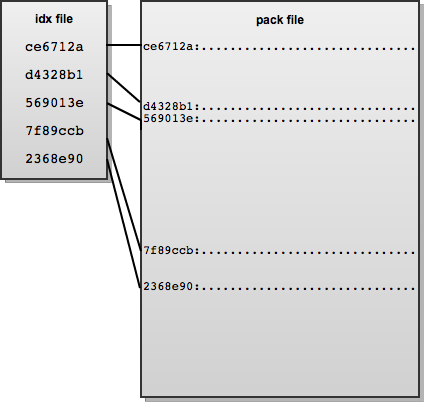
\includegraphics[width=0.6\textwidth]{gitPackFiles.png}
        \end{center}
    \end{frame}

    \begin{frame}
        \frametitle{Pack-файлы, подробности}
        \begin{itemize}
            \item Упаковка происходит, когда:
            \begin{itemize}
                \item Выполняется git push
                \item Слишком много <<свободных>> объектов (порядка 7000)
                \item Вручную вызвана git gc
            \end{itemize}
            \item Используется дельта-компрессия
            \begin{itemize}
                \item Последняя версия хранится целиком, дельты <<идут назад>>
            \end{itemize}
            \item Можно заглянуть внутрь, git verify-pack
            \item Git может хитро перепаковывать pack-файлы
        \end{itemize}
    \end{frame}

    \begin{frame}[fragile]
        \frametitle{Reflog и восстановление коммитов}
            \begin{minted}{text}
$ git reflog
1a410ef HEAD@{0}: reset: moving to 1a410ef
ab1afef HEAD@{1}: commit: modified repo.rb a bit
484a592 HEAD@{2}: commit: added repo.rb

$ git log -g
commit 1a410efbd13591db07496601ebc7a059dd55cfe9
Reflog: HEAD@{0} (Scott Chacon <schacon@gmail.com>)
Reflog message: updating HEAD
Author: Scott Chacon <schacon@gmail.com>
Date:   Fri May 22 18:22:37 2009 -0700

third commit
$ git branch recover-branch ab1afef
            \end{minted}
    \end{frame}

    \begin{frame}[fragile]
        \frametitle{Как более капитально прострелить себе ногу}
        \framesubtitle{И что делать}
        \begin{minted}{text}
$ git branch -D recover-branch
$ rm -Rf .git/logs/

$ git fsck --full
Checking object directories: 100% (256/256), done.
Checking objects: 100% (18/18), done.
dangling blob d670460b4b4aece5915caf5c68d12f560a9fe3e4
dangling commit ab1afef80fac8e34258ff41fc1b867c702daa24b
dangling tree aea790b9a58f6cf6f2804eeac9f0abbe9631e4c9
dangling blob 7108f7ecb345ee9d0084193f147cdad4d2998293
        \end{minted}
        Git не удалит даже <<висячие>> объекты несколько месяцев, если его явно не попросить.
    \end{frame}

    \begin{frame}
        \frametitle{Lessons Learned}
        \begin{itemize}
            \item Команды реализовывались как набор шелл-скриптов
            \begin{itemize}
                \item Не портировать под Windows
                \item Сложно интегрировать с IDE
                \item Замедлило внедрение git-а
            \end{itemize}
            \item Большой набор команд (включая plumbing) делает Git тяжёлым для изучения и усложняет сообщения об ошибках
        \end{itemize}
    \end{frame}

    \section{Mercurial}

    \begin{frame}
        \frametitle{Mercurial\footnote{\tiny{По \url{http://aosabook.org}}}}
        \begin{itemize}
            \item Python + C
            \item Распределённая VCS
            \item Architectural drivers
            \begin{itemize}
                \item Масштабные open-source-проекты (ядро Linux)
                \begin{itemize}
                    \item Миллионы файлов
                    \item Миллионы ревизий
                    \item Тысячи пользователей, вносящих изменения параллельно в течение десятилетий
                \end{itemize}
                \item Компрессия хранилища данных
                \item Эффективное получение произвольных ревизий
                \item Эффективное добавление новых ревизий
                \item Работа с историями файлов
            \end{itemize}
        \end{itemize}
    \end{frame}

    \begin{frame}
        \frametitle{Revlog}
        \begin{columns}
            \begin{column}{0.6\textwidth}
                \begin{itemize}
                    \item Каждый файл хранится в виде набора ревизий
                    \item Ревизии хранятся в виде дельт, иногда снапшоты файла целиком
                    \item Каждая ревизия описывается записью с форматом как на рисунке
                    \item Отдельно файл с дельтами (данные), отдельно файл с записями (индекс)
                    \item Сжатие zlib
                \end{itemize}
            \end{column}
            \begin{column}{0.4\textwidth}
                \begin{center}
                    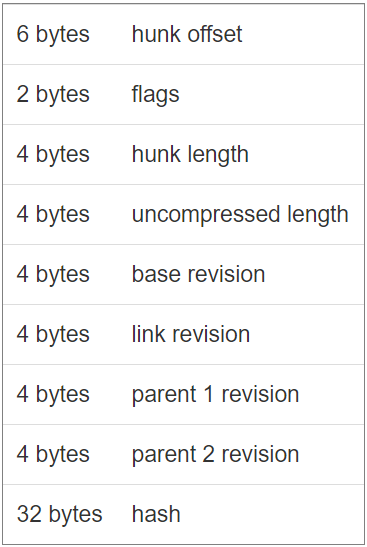
\includegraphics[width=0.8\textwidth]{revlog.png}
                \end{center}
            \end{column}
        \end{columns}
    \end{frame}

    \begin{frame}
        \frametitle{Структура revlog-ов}
        \begin{itemize}
            \item Сhangelog --- метаданные о ревизии + ссылка на манифест
            \item Manifests --- список имён файлов в ревизии + для каждого ссылка на filelog
            \item Filelog --- содержимое файлов ревизии + немного метаданных
            \item Dirstate --- информация о рабочей копии, кеш дерева файлов
            \item Обновление логов в фиксированном порядке, гарантирующее консистентность
            \item Revlog-и хранятся тоже в виде дельт
        \end{itemize}
        \begin{center}
            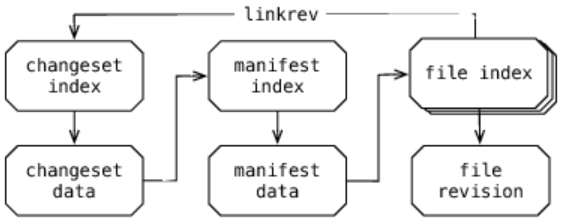
\includegraphics[width=0.5\textwidth]{mercurialLogStructure.png}
        \end{center}
    \end{frame}

    \begin{frame}[fragile]
        \frametitle{Как это выглядит}
        Changelog:
        \begin{minted}{text}
0a773e3480fe58d62dcc67bd9f7380d6403e26fa
Dirkjan Ochtman <dirkjan@ochtman.nl>
1276097267 -7200
mercurial/discovery.py
discovery: fix description line
        \end{minted}
        \vspace{3mm}
        Manifest:
        \begin{minted}{text}
.hgignore\x006d2dc16e96ab48b2fcca44f7e9f4b8c3289cb701
.hgsigs\x00de81f258b33189c609d299fd605e6c72182d7359
.hgtags\x00b174a4a4813ddd89c1d2f88878e05acc58263efa
CONTRIBUTORS\x007c8afb9501740a450c549b4b1f002c803c45193a
COPYING\x005ac863e17c7035f1d11828d848fb2ca450d89794
        \end{minted}
    \end{frame}

    \begin{frame}
        \frametitle{Ревизии}
        \begin{center}
            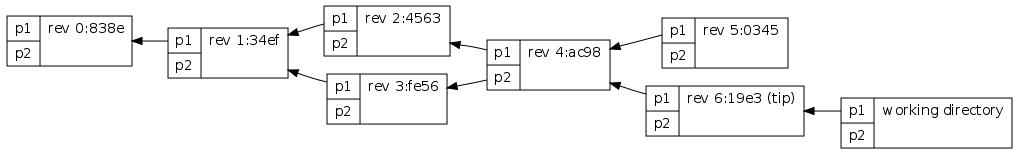
\includegraphics[width=\textwidth]{mercurialRevisions.png}
            \attribution{https://www.mercurial-scm.org/wiki/UnderstandingMercurial}
        \end{center}
        \begin{itemize}
            \item Локальный номер ревизии
            \begin{itemize}
                \item Доступ за константное время к узлу в revlog-е
            \end{itemize}
            \item Глобальный SHA-1-хеш ревизии
        \end{itemize}
    \end{frame}

    \begin{frame}
        \frametitle{Ветки}
        \begin{columns}
            \begin{column}{0.6\textwidth}
                \begin{enumerate}
                    \item Cоздание ветки через клонирование репозитория
                    \item Bookmarks --- объекты-ссылки в духе git
                    \item Именованные ветки --- имя ветки в метаданных ревизии
                    \item Анонимные ветки
                \end{enumerate}
                \begin{itemize}
                    \item Тэги хранятся как версионируемый файл .hgtags в репозитории
                \end{itemize}
            \end{column}
            \begin{column}{0.4\textwidth}
                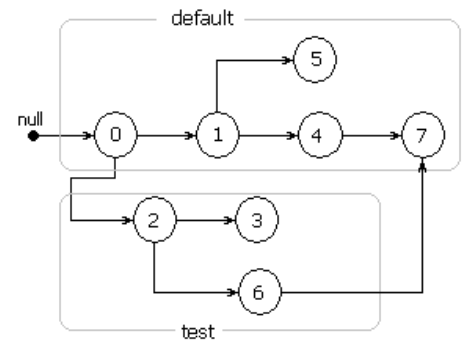
\includegraphics[width=\textwidth]{mercurialBranches.png}
            \end{column}
        \end{columns}
    \end{frame}

    \begin{frame}
        \frametitle{Статическая структура}
        \begin{columns}
            \begin{column}{0.4\textwidth}
                \begin{itemize}
                    \item Один модуль --- один файл
                    \item CLI
                    \item Одна команда --- одна функция, все в одном файле
                    \item Хеш-таблица, отображающая имена команд на функции
                    \item Опции, общие наборы опций
                \end{itemize}
            \end{column}
            \begin{column}{0.6\textwidth}
                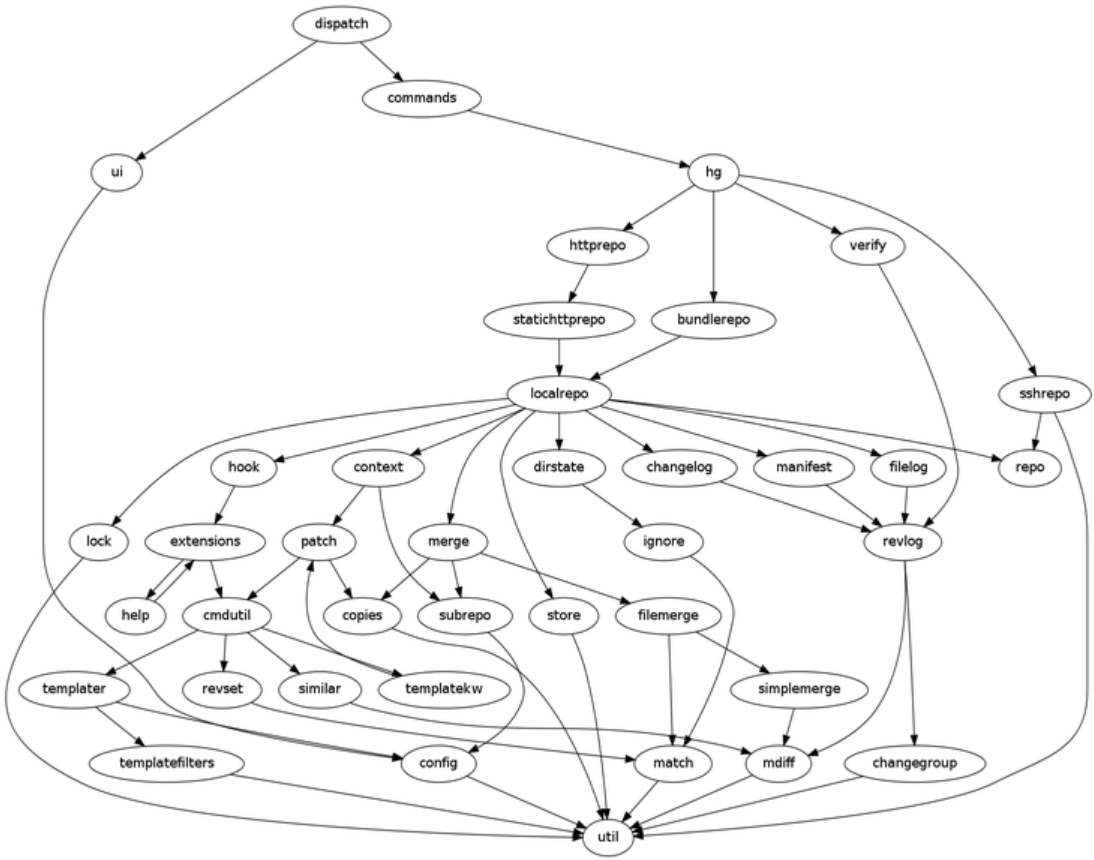
\includegraphics[width=\textwidth]{mercurialImportGraph.png}
            \end{column}
        \end{columns}
    \end{frame}

    \begin{frame}
        \frametitle{Расширяемость}
        \begin{itemize}
            \item Модули расширения
            \begin{itemize}
                \item Новые команды
                \begin{itemize}
                    \item cmdtable, uisetup, reposetup
                \end{itemize}
                \item Обёртки над существующими командами
                \item Обёртки над репозиторием
                \item Обёртки над любой функцией Mercurial
                \item Новые типы репозиториев (например, hgsubversion)
                \item Алиасы
            \end{itemize}
            \item hooks
            \begin{itemize}
                \item Вызов шелл-скрипта
                \item Вызов Python-функции
            \end{itemize}
        \end{itemize}
    \end{frame}

    \begin{frame}
        \frametitle{Lessons Learned}
        \begin{itemize}
            \item Python: и хорошо, и плохо
            \item Намеренно сложно модифицировать changeset после публикации, что плохо для локальной работы
            \item Revlogs + модель данных -- хорошо и эффективно, но не дружат с переименованиями
            \item Небольшое количество основных команд помогает легче научиться
            \item .hgtags оказался внезапен для пользователей
            \item Люди впервые знакомились с Python, чтобы писать расширения для mercurial, потому что это просто
        \end{itemize}
    \end{frame}

    \section{Subversion}

    \begin{frame}
        \frametitle{Subversion\footnote{\tiny{По \url{http://svnbook.red-bean.com/en/1.7/svn-book.html}}}}
        \begin{itemize}
            \item Написана на C
            \item Централизованная VCS
            \item Architectural drivers
            \begin{itemize}
                \item починить CVS
                \item не поддерживать обратную совместимость с CVS, но сделать переход по возможности безболезненным
                \item развивать проект как open source
            \end{itemize}
        \end{itemize}
    \end{frame}

    \begin{frame}
        \frametitle{Архитектура}
        \begin{center}
            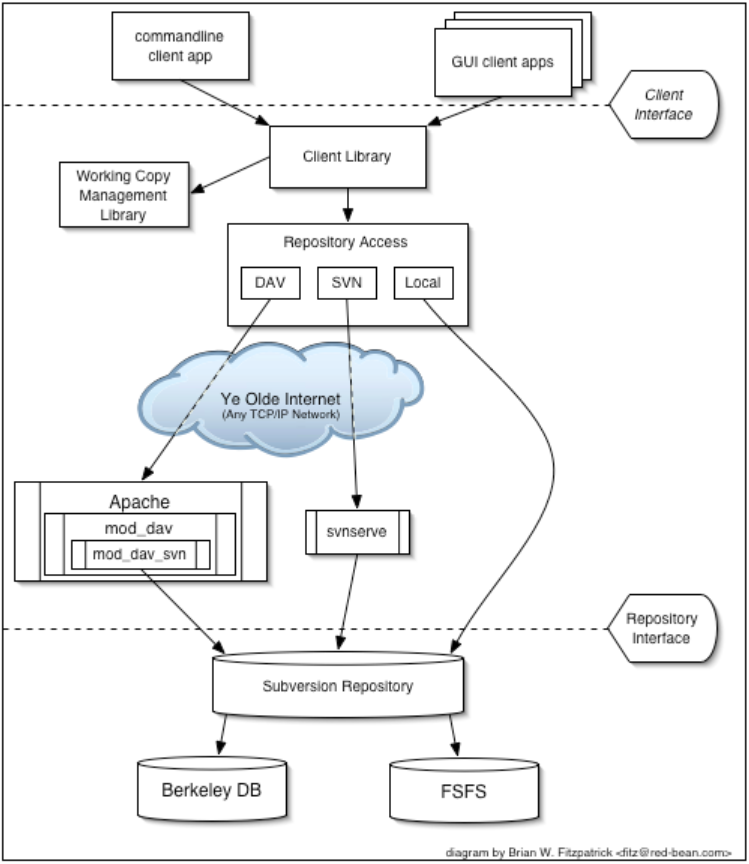
\includegraphics[height=0.8\textheight]{subversionArchitecture.png}
        \end{center}
    \end{frame}

    \begin{frame}
        \frametitle{Ревизии и репозиторий}
        \begin{itemize}
            \item Ревизии имеют уникальный числовой номер
            \begin{itemize}
                \item Хранятся в виде обратных дельт со снапшотами
            \end{itemize}
            \item Номер ревизии --- свойство всего репозитория, а не файла
            \item В рабочей копии ревизии разных файлов могут быть разными
            \item Коммиты атомарны
            \item Единое дерево исходников
            \begin{itemize}
                \item trunk
                \item branches
                \item tags
            \end{itemize}
            \item Ветка и тэг --- не более чем копия папки
            \item Репозиторий не хранит копии одного файла
            \item Можно чекаутить конкретную папку
        \end{itemize}
    \end{frame}

    \begin{frame}
        \frametitle{Структура репозитория}
        \begin{itemize}
            \item conf/ --- папка с конфигурационными файлами
            \item db/ --- хранилище версионируемых данных
            \begin{itemize}
                \item BerkleyDB или FSFS
            \end{itemize}
            \item format --- описывает организацию репозитория
            \item hooks/ --- папка со скриптами-хуками
            \item locks/ --- замки для управления одновременным доступом
            \item README.txt --- файл, в котором написано, что это репозиторий Subversion
        \end{itemize}
    \end{frame}

    \begin{frame}[fragile]
        \frametitle{Свойства}
        \begin{itemize}
            \item Свойства --- пары ``ключ-значение'', которые хранятся вместе с файлами, папками или ревизиями
            \item Ключ --- строка из ASCII-символов, значение --- либой массив байтов
            \item Версионируются как данные в самих файлах
            \item Активно используются самой Subversion и тулами
            \begin{itemize}
                \item Например, \verb|svn:ignore|, \verb|svn:eol-style|
            \end{itemize}
            \item Например, для набора изображений можно хранить в свойствах описание, дату и даже thumbnail
        \end{itemize}
    \end{frame}

    \begin{frame}[fragile]
        \frametitle{Проблемы и ограничения}
        % См. https://en.wikipedia.org/wiki/Apache_Subversion
        \begin{itemize}
            \item Переименование реализовано как copy и delete, что смущает разрешение конфликтов
            \item До версии 1.7 папки .svn хранились в каждой папке проекта
            \item При чекауте не выставляются ``настоящие'' времена модификации файлов, используется время чекаута
            \begin{itemize}
                \item Неожиданно для пользователя, но полезно для make
            \end{itemize}
            \item ``Наивная'' поддержка веток и тэгов, делает невозможными некоторые операции
            \begin{itemize}
                \item Например, \verb|svn log -r tag1:tag2 myfile|
            \end{itemize}
        \end{itemize}
    \end{frame}

\end{document}
